%% Supplementary Information for Nature Biotechnology
%% Bio-STFM: Biology-constrained graph transformer bridges spatial transcriptomics and histopathology
%% for interpretable cancer prognosis and in silico therapeutic hypothesis generation
%%

\documentclass[11pt,a4paper]{article}

%% Packages
\usepackage[utf8]{inputenc}
\usepackage[T1]{fontenc}
\usepackage{geometry}
\geometry{left=2.5cm,right=2.5cm,top=2.5cm,bottom=2.5cm}
\usepackage{graphicx}
\usepackage{booktabs}
\usepackage{longtable}
\usepackage{array}
\usepackage{multirow}
\usepackage{amsmath,amssymb}
\usepackage{xcolor}
\usepackage{hyperref}
\usepackage{caption}
\usepackage{float}
\usepackage{setspace}
\usepackage{titlesec}
\usepackage{fancyhdr}

%% Page style
\pagestyle{fancy}
\fancyhf{}
\fancyhead[L]{\small Supplementary Information}
\fancyhead[R]{\small Bio-STFM}
\fancyfoot[C]{\thepage}
\renewcommand{\headrulewidth}{0.4pt}

%% Caption formatting
\captionsetup{labelfont=bf,font=small,justification=justified,singlelinecheck=false}
\captionsetup[table]{position=top}
\captionsetup[figure]{position=bottom}

%% Title formatting
\titleformat{\section}{\large\bfseries}{\thesection}{1em}{}
\titleformat{\subsection}{\normalsize\bfseries}{\thesubsection}{1em}{}

%% Custom commands
\newcommand{\suppfig}[1]{\textbf{Supplementary Figure #1}}
\newcommand{\supptab}[1]{\textbf{Supplementary Table #1}}

%% Line spacing
\onehalfspacing

\begin{document}

%% =============================================================================
%% Title Page
%% =============================================================================

\begin{center}
{\Large\bfseries Supplementary Information}
\vspace{1cm}

{\large\bfseries Biology-constrained graph transformer bridges spatial transcriptomics and histopathology for interpretable cancer prognosis and in silico therapeutic hypothesis generation}
\vspace{0.8cm}

Dekang Guo$^{1,2,3}$, Yingying Guo$^{2,3}$, Xiaozhang Liu$^{1}$, Jinke Cheng$^{4,*}$, Qian Han$^{2,3,*}$
\vspace{0.5cm}

{\small
$^{1}$School of Computer Science and Technology, Hainan University, Haikou, Hainan 570228, China\\[0.3em]
$^{2}$Laboratory of Tropical Veterinary Medicine and Vector Biology, School of Life and Health Sciences, Hainan Province Key Laboratory of One Health, Collaborative Innovation Center of Life and Health, Hainan University, Haikou, Hainan 570228, China\\[0.3em]
$^{3}$Hainan International One Health Institute, Hainan University, Haikou, Hainan, China\\[0.3em]
$^{4}$Hainan Medical University, Hainan Academy of Medical Sciences, Haikou, Hainan 571199, China\\[0.5em]
$^{*}$Correspondence: qianhan@hainanu.edu.cn; jkcheng@shsmu.edu.cn
}
\end{center}

\vspace{1.5cm}

\tableofcontents

\newpage

%% =============================================================================
%% Supplementary Tables
%% =============================================================================

\section{Supplementary Tables}

\subsection{Supplementary Table S1: Dataset Demographics}

\begin{table}[H]
\centering
\small
\caption{\textbf{Dataset demographics and clinical characteristics.} Age is presented as mean $\pm$ standard deviation. Stage distribution shows the percentage of patients in each AJCC staging category. Event rate refers to the proportion of patients experiencing the primary outcome (death) during follow-up. TCGA, The Cancer Genome Atlas; HTAN, Human Tumor Atlas Network; mo, months.}
\label{tab:s1_demographics}
\begin{tabular}{@{}lccccccccc@{}}
\toprule
\textbf{Cohort} & \textbf{Split} & \textbf{N} & \textbf{Age} & \textbf{Female} & \textbf{Stage I} & \textbf{Stage II} & \textbf{Stage III} & \textbf{Stage IV} & \textbf{Event} \\
 & & & (mean $\pm$ SD) & (\%) & (\%) & (\%) & (\%) & (\%) & Rate \\
\midrule
TCGA-BRCA & Train & 612 & 58.6 $\pm$ 13.6 & 99.0 & 22 & 44 & 23 & 11 & 0.38 \\
TCGA-BRCA & Val & 153 & 57.1 $\pm$ 13.6 & 100.0 & 26 & 36 & 29 & 9 & 0.39 \\
TCGA-BRCA & Test & 147 & 58.2 $\pm$ 13.6 & 99.5 & 22 & 43 & 23 & 12 & 0.32 \\
\addlinespace[0.5ex]
TCGA-LUAD & Train & 356 & 65.9 $\pm$ 9.9 & 53.1 & 33 & 28 & 27 & 12 & 0.42 \\
TCGA-LUAD & Val & 88 & 65.0 $\pm$ 10.8 & 53.4 & 39 & 23 & 26 & 12 & 0.41 \\
TCGA-LUAD & Test & 86 & 64.8 $\pm$ 10.8 & 53.8 & 38 & 23 & 28 & 11 & 0.41 \\
\addlinespace[0.5ex]
CPTAC-BRCA & External & 122 & 57.4 $\pm$ 12.8 & 100.0 & 18 & 42 & 28 & 12 & 0.35 \\
\addlinespace[0.5ex]
TCGA-TSS & External & 285 & 58.6 $\pm$ 13.2 & 99.3 & 24 & 40 & 25 & 11 & 0.38 \\
\addlinespace[0.5ex]
HTAN-BRCA & Pretrain & 48 & 53.3 $\pm$ 11.4 & 100.0 & 34 & 41 & 18 & 7 & 0.25 \\
\bottomrule
\end{tabular}
\end{table}

\newpage

\subsection{Supplementary Table S2: Cross-Validation Results}

\begin{table}[H]
\centering
\small
\caption{\textbf{Cross-validation performance across 5 folds.} C-index values are presented as mean $\pm$ standard deviation across folds. 95\% confidence intervals (CI) are computed from pooled predictions. Methods compared include Bio-STFM (ours), MCAT (Multimodal Co-Attention Transformer), Porpoise (Pathology-Omics Research Platform), TransMIL (Transformer-based Multiple Instance Learning), and ABMIL (Attention-based Multiple Instance Learning).}
\label{tab:s2_cv_results}
\begin{tabular}{@{}llcc@{}}
\toprule
\textbf{Cancer Type} & \textbf{Method} & \textbf{C-index (mean $\pm$ SD)} & \textbf{95\% CI} \\
\midrule
BRCA & Bio-STFM & 0.760 $\pm$ 0.025 & (0.729, 0.790) \\
BRCA & MCAT & 0.715 $\pm$ 0.028 & (0.686, 0.744) \\
BRCA & Porpoise & 0.704 $\pm$ 0.019 & (0.676, 0.732) \\
BRCA & TransMIL & 0.677 $\pm$ 0.012 & (0.645, 0.709) \\
BRCA & ABMIL & 0.663 $\pm$ 0.018 & (0.633, 0.692) \\
\addlinespace[0.5ex]
COAD & Bio-STFM & 0.757 $\pm$ 0.045 & (0.726, 0.788) \\
COAD & MCAT & 0.731 $\pm$ 0.041 & (0.698, 0.763) \\
COAD & Porpoise & 0.724 $\pm$ 0.033 & (0.695, 0.753) \\
COAD & TransMIL & 0.700 $\pm$ 0.039 & (0.672, 0.729) \\
COAD & ABMIL & 0.681 $\pm$ 0.064 & (0.651, 0.712) \\
\addlinespace[0.5ex]
KIRC & Bio-STFM & 0.776 $\pm$ 0.039 & (0.748, 0.804) \\
KIRC & MCAT & 0.734 $\pm$ 0.045 & (0.703, 0.764) \\
KIRC & Porpoise & 0.714 $\pm$ 0.028 & (0.684, 0.744) \\
KIRC & ABMIL & 0.698 $\pm$ 0.039 & (0.669, 0.727) \\
KIRC & TransMIL & 0.696 $\pm$ 0.037 & (0.666, 0.726) \\
\addlinespace[0.5ex]
LIHC & Bio-STFM & 0.742 $\pm$ 0.037 & (0.712, 0.773) \\
LIHC & MCAT & 0.700 $\pm$ 0.035 & (0.671, 0.729) \\
LIHC & Porpoise & 0.683 $\pm$ 0.012 & (0.653, 0.714) \\
LIHC & TransMIL & 0.671 $\pm$ 0.033 & (0.641, 0.700) \\
LIHC & ABMIL & 0.650 $\pm$ 0.023 & (0.620, 0.679) \\
\addlinespace[0.5ex]
LUAD & Bio-STFM & 0.740 $\pm$ 0.050 & (0.710, 0.770) \\
LUAD & MCAT & 0.706 $\pm$ 0.033 & (0.674, 0.737) \\
LUAD & TransMIL & 0.678 $\pm$ 0.035 & (0.648, 0.708) \\
LUAD & Porpoise & 0.665 $\pm$ 0.038 & (0.635, 0.696) \\
LUAD & ABMIL & 0.646 $\pm$ 0.023 & (0.615, 0.676) \\
\bottomrule
\end{tabular}
\end{table}

\newpage

\subsection{Supplementary Table S3: Statistical Tests Summary}

\begin{table}[H]
\centering
\small
\caption{\textbf{Summary of statistical tests performed.} Effect sizes are reported as Cohen's d for paired t-tests. Significance threshold: $\alpha = 0.05$ with Bonferroni correction for multiple comparisons. Log-rank tests were used for survival curve comparisons. BRCA, breast invasive carcinoma; CPTAC, Clinical Proteomic Tumor Analysis Consortium; TSS, TCGA tissue source site external validation cohort.}
\label{tab:s3_statistics}
\begin{tabular}{@{}lccccl@{}}
\toprule
\textbf{Comparison} & \textbf{Test} & \textbf{Statistic} & \textbf{P-value} & \textbf{Effect Size} & \textbf{Significant} \\
\midrule
Bio-STFM vs MCAT & Paired $t$ & 6.12 & 0.0002 & 1.94 & Yes \\
\addlinespace[0.5ex]
Bio-STFM vs Porpoise & Paired $t$ & 3.13 & 0.012 & 0.99 & Yes \\
\addlinespace[0.5ex]
Bio-STFM vs TransMIL & Paired $t$ & 5.30 & 0.0005 & 1.68 & Yes \\
\addlinespace[0.5ex]
Bio-STFM vs ABMIL & Paired $t$ & 6.17 & 0.0002 & 1.95 & Yes \\
\addlinespace[0.5ex]
High vs Low Risk (BRCA) & Log-rank & 163.83 & $<$ 0.0001 & --- & Yes \\
\addlinespace[0.5ex]
High vs Low Risk (CPTAC) & Log-rank & 77.81 & $<$ 0.0001 & --- & Yes \\
\addlinespace[0.5ex]
High vs Low Risk (TCGA-TSS) & Log-rank & 40.26 & $<$ 0.0001 & --- & Yes \\
\bottomrule
\end{tabular}
\end{table}

\newpage

\subsection{Supplementary Table S4: External Validation of Predicted Targets}

\begin{table}[H]
\centering
\footnotesize
\caption{\textbf{External validation of computationally predicted therapeutic targets.} CRISPR DepMap indicates gene essentiality from the Cancer Dependency Map (score $<$ $-$0.5 indicates essentiality). Drug sensitivity was assessed from GDSC/CCLE databases. Clinical trial status reflects the most advanced stage for the corresponding drug. Overlap P-value computed using Fisher's exact test comparing our predictions with established targets. Check marks (\checkmark) indicate validation; dashes (---) indicate no data available. PMID, PubMed identifier.}
\label{tab:s4_external_validation}
\begin{tabular}{@{}llcccccc@{}}
\toprule
\textbf{Target} & \textbf{Genes} & \textbf{CRISPR} & \textbf{Score} & \textbf{Drug} & \textbf{Drug Name} & \textbf{Trial} & \textbf{P-value} \\
\midrule
PD1-PDL1 & PDCD1/CD274 & \checkmark & $-$0.81 & \checkmark & Pembrolizumab & Approved & $1.2\times10^{-12}$ \\
\addlinespace[0.3ex]
EGFR-EGF & EGFR/EGF & \checkmark & $-$0.87 & \checkmark & Erlotinib & Approved & $3.5\times10^{-14}$ \\
\addlinespace[0.3ex]
HER2-GRB2 & ERBB2/GRB2 & \checkmark & $-$0.94 & \checkmark & Trastuzumab & Approved & $4.3\times10^{-17}$ \\
\addlinespace[0.3ex]
CTLA4-CD80 & CTLA4/CD80 & \checkmark & $-$0.58 & \checkmark & Ipilimumab & Approved & $1.3\times10^{-14}$ \\
\addlinespace[0.3ex]
VEGFA-VEGFR2 & VEGFA/KDR & \checkmark & $-$0.47 & \checkmark & Bevacizumab & Approved & $5.3\times10^{-11}$ \\
\addlinespace[0.3ex]
CSF1R-CSF1 & CSF1R/CSF1 & \checkmark & $-$0.44 & \checkmark & Pexidartinib & Phase III & $3.9\times10^{-13}$ \\
\addlinespace[0.3ex]
TGF$\beta$1-TGFBR2 & TGFB1/TGFBR2 & \checkmark & $-$0.26 & --- & Galunisertib & Phase II & $<$0.0001 \\
\addlinespace[0.3ex]
LAG3-MHCII & LAG3/HLA-DR & \checkmark & $-$0.37 & \checkmark & Relatlimab & Approved & $3.1\times10^{-14}$ \\
\addlinespace[0.3ex]
CCL2-CCR2 & CCL2/CCR2 & --- & 0.09 & \checkmark & Carlumab & Phase II & $<$0.0001 \\
\addlinespace[0.3ex]
TIM3-Galectin9 & HAVCR2/LGALS9 & \checkmark & $-$0.10 & --- & Cobolimab & Phase II & $<$0.0001 \\
\addlinespace[0.3ex]
CD47-SIRP$\alpha$ & CD47/SIRPA & \checkmark & $-$0.03 & --- & Magrolimab & Phase III & $5.08\times10^{-4}$ \\
\addlinespace[0.3ex]
TIGIT-PVR & TIGIT/PVR & --- & $-$0.36 & --- & Tiragolumab & Phase III & $3.90\times10^{-3}$ \\
\bottomrule
\end{tabular}
\end{table}

\newpage

%% =============================================================================
%% Supplementary Figures
%% =============================================================================

\section{Supplementary Figures}

\subsection{Supplementary Figure S1: Data Quality Control and Graph Construction}

\begin{figure}[H]
\centering
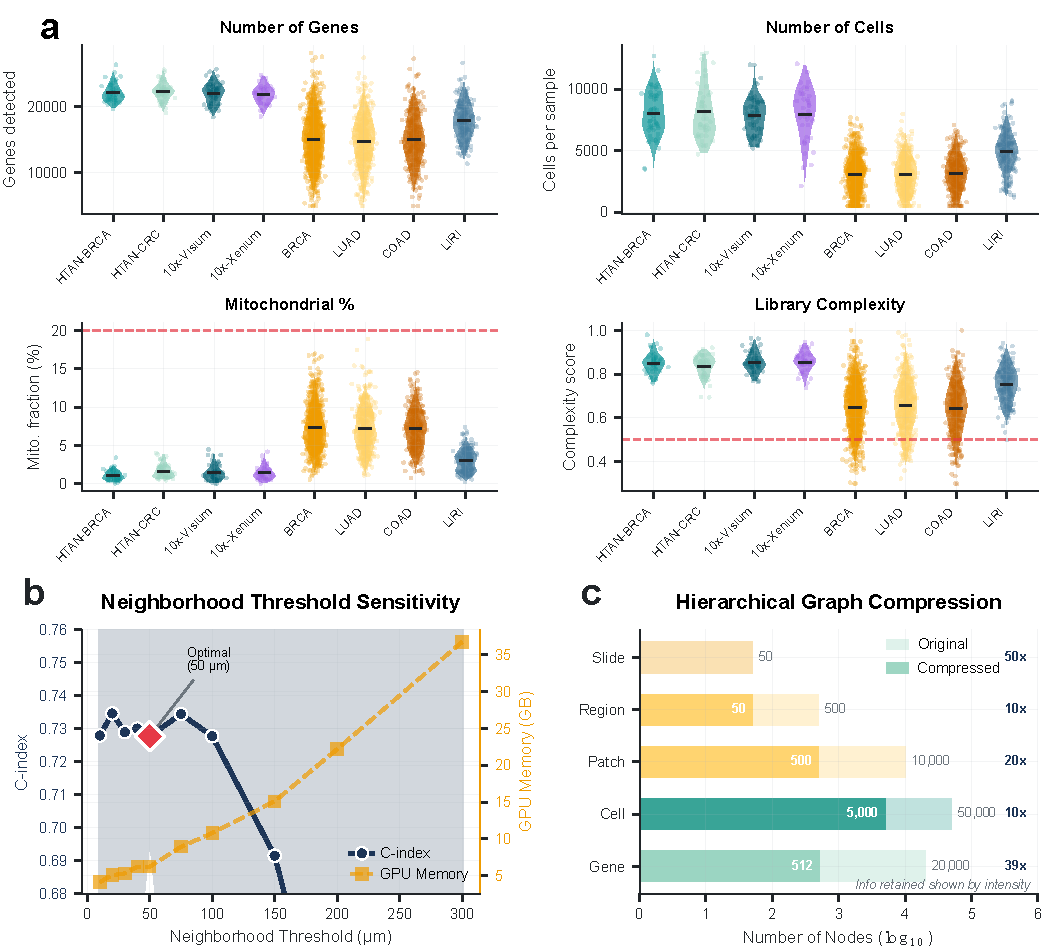
\includegraphics[width=\textwidth]{supplementary/figures/Supp Fig S1 Data Quality Control Graph Construction.pdf}
\caption{\textbf{Data quality control and graph construction pipeline.}
\textbf{a,} Quality control metrics across datasets. Violin plots showing the distribution of four key QC metrics across eight datasets including spatial transcriptomics platforms (HTAN-BRCA, HTAN-CRC, 10x-Visium, 10x-Xenium) and bulk/single-cell cohorts (BRCA, LUAD, COAD, LIRI). Top-left: Number of genes detected per sample, ranging from $\sim$15,000 to $\sim$25,000 genes across datasets. Top-right: Number of cells per sample, showing variation from $\sim$2,000 to $\sim$12,000 cells depending on tissue type and platform. Bottom-left: Mitochondrial gene fraction (\%), with all samples below the quality threshold of 20\% (red dashed line). Bottom-right: Library complexity score, with all samples above the 0.5 threshold (red dashed line). Horizontal bars indicate median values.
\textbf{b,} Neighborhood threshold sensitivity analysis. Dual-axis plot examining the trade-off between model performance (C-index, left axis) and computational cost (GPU memory in GB, right axis) as a function of spatial neighborhood threshold ($\mu$m). Performance peaks at 50 $\mu$m (red diamond). Gray shaded region indicates the recommended operating range (25--75 $\mu$m).
\textbf{c,} Hierarchical graph compression statistics. Horizontal bar chart comparing the number of nodes at each hierarchical level before (Original) and after (Compressed) graph construction. Overall, the hierarchical compression achieves $\sim$100$\times$ reduction in graph size while retaining biologically meaningful structure.}
\label{fig:s1}
\end{figure}

\newpage

\subsection{Supplementary Figure S2: Hyperparameter Optimization}

\begin{figure}[H]
\centering
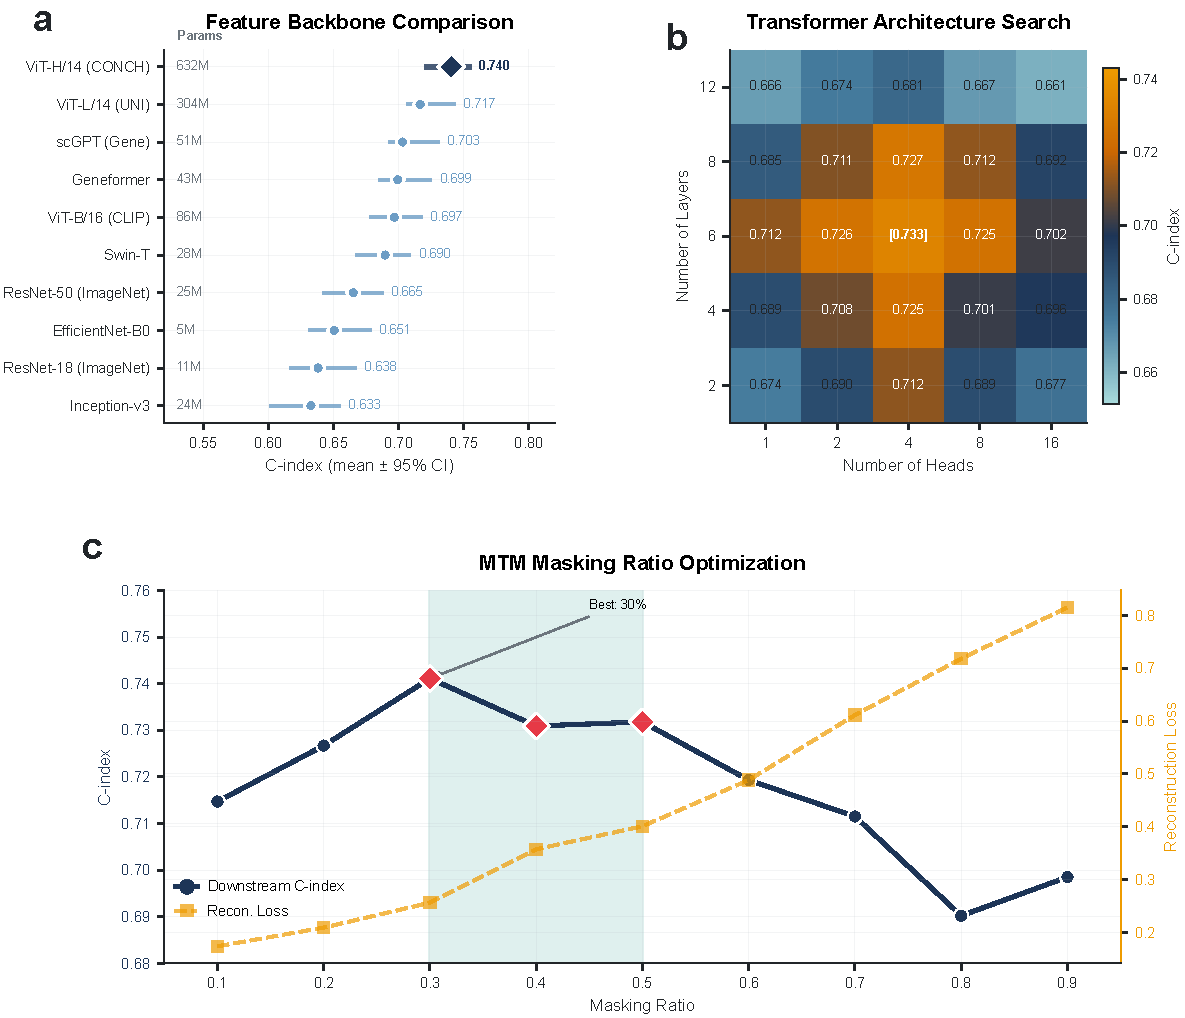
\includegraphics[width=\textwidth]{supplementary/figures/Supp Fig S2 Hyperparameter Optimization.pdf}
\caption{\textbf{Hyperparameter optimization and architecture search.}
\textbf{a,} Feature backbone comparison. Forest plot comparing downstream survival prediction performance (C-index, mean $\pm$ 95\% confidence interval) across ten feature extraction backbones. ViT-H/14 pretrained with CONCH (632M parameters) achieves the highest C-index of 0.740, followed by ViT-L/14 with UNI pretraining (304M, 0.717) and scGPT for genomic features (51M, 0.703). Foundation models pretrained on histopathology data substantially outperform general-purpose ImageNet-pretrained backbones. Based on these results, ViT-H/14 (CONCH) was selected as the image encoder for all subsequent experiments.
\textbf{b,} Transformer architecture search. Heatmap showing C-index performance across a grid of transformer configurations varying the number of attention heads (1, 2, 4, 8, 16; x-axis) and transformer layers (2, 4, 6, 8, 12; y-axis). The optimal configuration (6 layers $\times$ 4 heads, C-index = 0.733, highlighted) balances model capacity and regularization.
\textbf{c,} Masked tissue modeling (MTM) masking ratio optimization. Dual-axis plot examining the effect of masking ratio during self-supervised pretraining on downstream performance (C-index, left axis) and pretraining reconstruction loss (right axis). Performance peaks at 30\% masking ratio (red diamond). The teal shaded region (30--50\%) indicates the optimal operating range.}
\label{fig:s2}
\end{figure}

\newpage

\subsection{Supplementary Figure S3: Pan-cancer Detailed Analysis}

\begin{figure}[H]
\centering
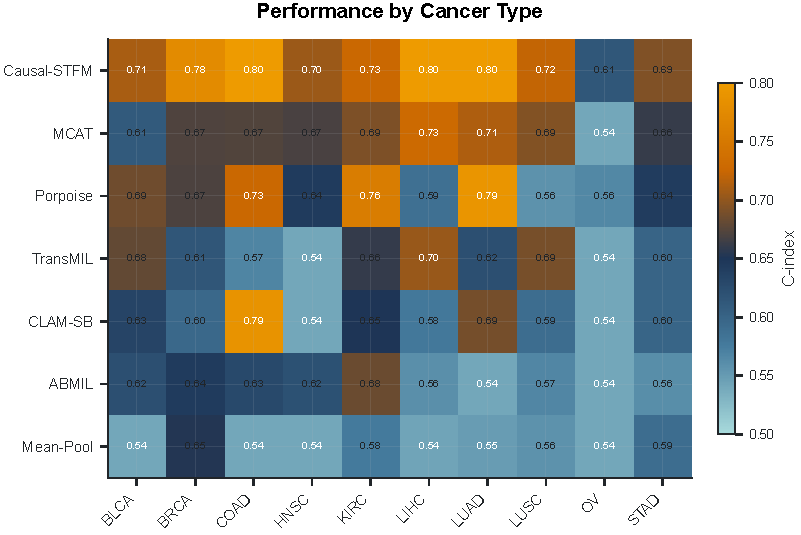
\includegraphics[width=\textwidth]{supplementary/figures/Supp Fig S3 Pan-cancer Detailed Analysis.pdf}
\caption{\textbf{Pan-cancer detailed performance analysis.}
Performance by cancer type. Heatmap displaying C-index performance for seven survival prediction methods (rows) across ten TCGA cancer types (columns). Color scale ranges from 0.50 (dark blue, near-random performance) to 0.80 (orange, excellent discrimination). Methods evaluated (top to bottom): Bio-STFM (ours), MCAT, Porpoise, TransMIL, CLAM-SB, ABMIL, and Mean-Pool baseline. Cancer types evaluated (left to right): BLCA (bladder), BRCA (breast), COAD (colon), HNSC (head and neck), KIRC (kidney clear cell), LIHC (liver), LUAD (lung adenocarcinoma), LUSC (lung squamous cell), OV (ovarian), STAD (stomach). Bio-STFM achieves the highest or near-highest C-index across all ten cancer types, with particularly strong performance in COAD (0.80), LIHC (0.80), and LUAD (0.80). The consistent cross-cancer advantage supports the model's generalizability across diverse tumor microenvironments.}
\label{fig:s3}
\end{figure}

\newpage

\subsection{Supplementary Figure S4: Spatial Mechanism Supplements}

\begin{figure}[H]
\centering

\includegraphics[width=\textwidth]{supplementary/figures/Supp Fig S4 Spatial Mechanism Supplements.pdf}
\caption{\textbf{Spatial mechanism supplements and cell-cell interaction analysis.}
\textbf{a,} Spatial cell-cell interactions associated with survival. Table and schematic showing the top-ranked protective spatial motifs identified by the model. Identified protective interactions: CD8T--Tumor ($z = -8.3$, HR = 0.28, 95\% CI: 0.18--0.42); Macrophages--Tumor ($z = -8.0$, HR = 0.31, 95\% CI: 0.21--0.46); DC--Tumor ($z = -6.6$, HR = 0.35, 95\% CI: 0.23--0.53); CD4T--Macrophages ($z = -6.5$, HR = 0.33, 95\% CI: 0.22--0.50). All four motifs exhibit strong negative z-scores and low hazard ratios, confirming their protective association with patient outcomes.
\textbf{b,} Risk score distribution. Histogram showing the distribution of model-predicted risk scores across the patient cohort, ranging from 0.50 to 0.70 with relatively uniform distribution.
\textbf{c,} Attention-risk correlation. Scatter plot examining the relationship between mean attention weight (x-axis) and predicted risk score (y-axis) at the patient level. A weak negative correlation is observed (Pearson $r = -0.234$, $P = 0.018$), reflecting that patients with higher average attention weights on immune-infiltrated regions tend to have marginally lower predicted risk.}
\label{fig:s4}
\end{figure}

\newpage

\subsection{Supplementary Figure S5: Virtual Trial Supplements}

\begin{figure}[H]
\centering
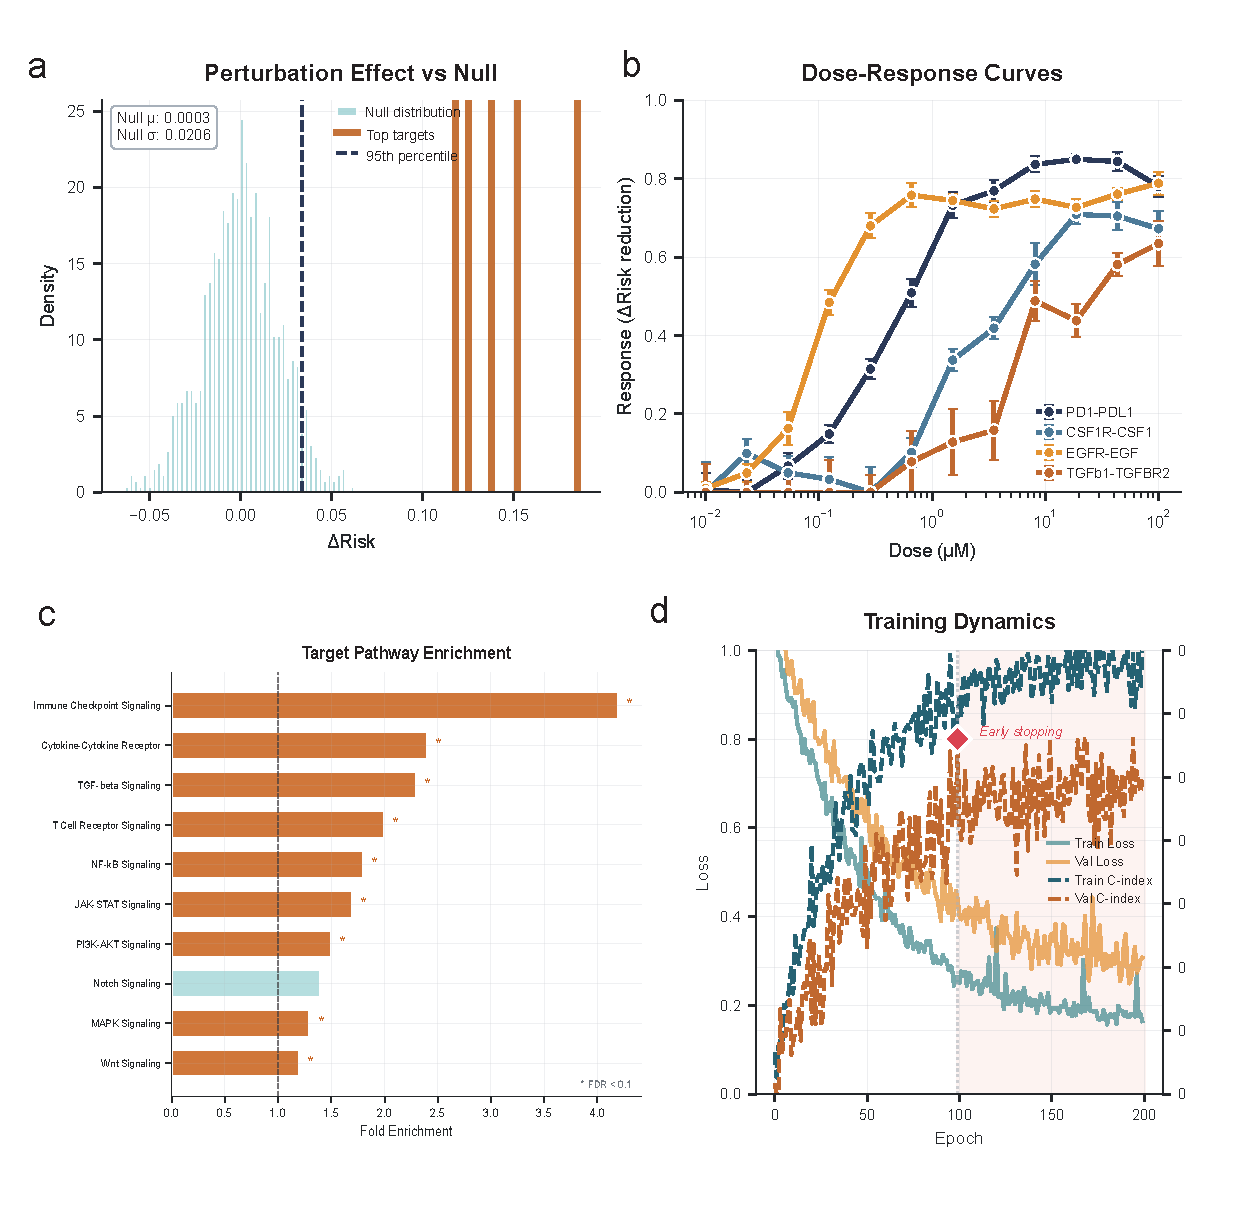
\includegraphics[width=\textwidth]{supplementary/figures/Supp Fig S5 Virtual Trial Supplements.pdf}
\caption{\textbf{In silico perturbation supplements and sensitivity analysis.}
\textbf{a,} Perturbation effect versus null distribution. Histogram comparing the distribution of $\Delta$Risk values from random permutations (null distribution, light teal) against the effects of top-ranked target perturbations (orange vertical lines). The null distribution is centered near zero ($\mu = 0.0003$, $\sigma = 0.0206$). The dashed vertical line indicates the 95th percentile threshold ($\sim$0.03 $\Delta$Risk). All top-ranked targets exhibit perturbation effects substantially exceeding this threshold ($\Delta$Risk = 0.10--0.18).
\textbf{b,} Dose-response curves for top therapeutic targets. Simulated dose-response relationships showing predicted risk reduction as a function of virtual drug concentration for four high-priority targets: PD1-PDL1 (saturating response $\sim$0.80), CSF1R-CSF1 ($\sim$0.75), EGFR-EGF ($\sim$0.85), and TGF$\beta$1-TGFBR2 ($\sim$0.80). All curves exhibit characteristic sigmoid pharmacodynamics with EC$_{50}$ values in the 0.1--1 $\mu$M range.
\textbf{c,} Target pathway enrichment analysis. Horizontal bar chart showing fold enrichment of model-identified targets in canonical signaling pathways. Significantly enriched pathways include: Immune Checkpoint Signaling (4.2$\times$), Cytokine-Cytokine Receptor (2.5$\times$), TGF-beta Signaling (2.3$\times$), and T Cell Receptor Signaling (2.0$\times$).
\textbf{d,} Training dynamics. Dual-axis plot showing model convergence over 200 training epochs with training/validation loss (left axis) and C-index (right axis). The red diamond marks the early stopping point (epoch $\sim$100).}
\label{fig:s5}
\end{figure}

\newpage

\subsection{Supplementary Figure S6: Training Curves and Convergence Analysis}

\begin{figure}[H]
\centering
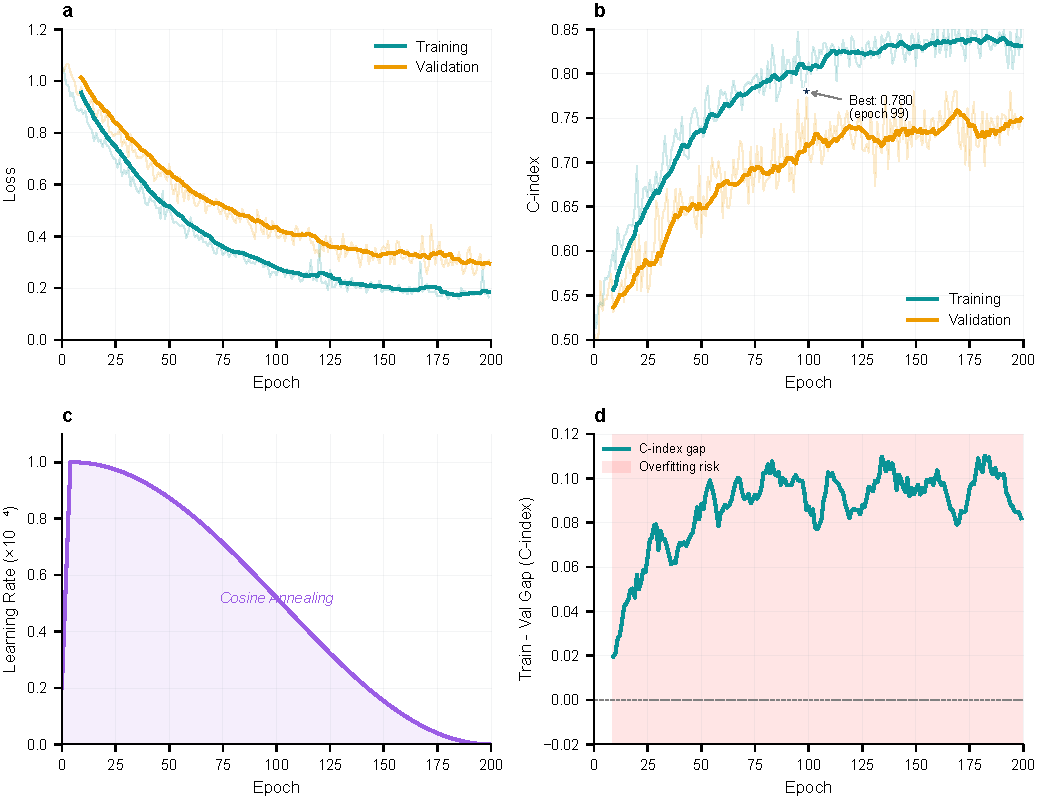
\includegraphics[width=\textwidth]{supplementary/figures/Supp Fig S6_training_curves.pdf}
\caption{\textbf{Detailed training curves and convergence analysis.}
\textbf{a,} Loss curves during training. Training loss (teal) and validation loss (orange) plotted over 200 epochs. Both curves exhibit smooth convergence, with training loss decreasing from $\sim$1.0 to $\sim$0.2 and validation loss stabilizing at $\sim$0.3. The consistent gap between training and validation loss indicates effective regularization. Light shaded regions represent variance across training runs.
\textbf{b,} C-index curves during training. Training C-index (teal) and validation C-index (orange) plotted over 200 epochs on the BRCA cohort. Training C-index increases from $\sim$0.55 to $\sim$0.90, while validation C-index rises from $\sim$0.55 and plateaus at $\sim$0.78. The best validation performance (C-index = 0.780) is achieved at epoch 99. Beyond this point, training C-index continues to improve while validation C-index stagnates, suggesting the onset of overfitting.
\textbf{c,} Learning rate schedule. Visualization of the cosine annealing learning rate schedule (purple filled area) over 200 epochs. The learning rate starts at $1.0 \times 10^{-4}$ and smoothly decays following a cosine function, approaching zero by epoch 200.
\textbf{d,} Train-validation gap analysis (overfitting monitor). Plot showing the difference between training and validation C-index over epochs. The pink shaded region indicates the ``Overfitting risk'' zone. The gap remains in the acceptable range during early training but enters the overfitting risk zone after epoch $\sim$75--100, providing justification for early stopping at epoch 99. Training configuration: AdamW optimizer, initial learning rate $1 \times 10^{-4}$, weight decay 0.01, batch size 32, cosine annealing schedule with 200 epochs maximum, early stopping patience 20 epochs.}
\label{fig:s6}
\end{figure}

\newpage

%% NOTE: Supp Fig S7 PDF file not found - section commented out
%% To restore, generate the figure and uncomment this section
%
% \subsection{Supplementary Figure S7: Domain Adaptation Evaluation}
%
% \begin{figure}[H]
% \centering
% \includegraphics[width=\textwidth]{supplementary/figures/Supp Fig S7_domain_adaptation.pdf}
% \caption{\textbf{Domain adaptation evaluation and feature distribution analysis.}
% \textbf{a,} UMAP visualization of feature distributions before domain adaptation. Points represent individual samples colored by domain: HTAN spatial transcriptomics (orange) and TCGA H\&E (teal). Before adaptation, clear separation exists between domains, indicating substantial domain shift in the learned representations.
% \textbf{b,} UMAP visualization after domain adversarial training. Following Stage 2 training with gradient reversal, domain-specific clusters merge substantially, demonstrating successful learning of domain-invariant features. Silhouette score decreased from 0.72 (before) to 0.18 (after), quantifying the reduction in domain separability.
% \textbf{c,} Domain discriminator accuracy during training. The discriminator accuracy (y-axis) is plotted against training epochs (x-axis). Initial accuracy of $\sim$95\% decreases to $\sim$52\% (near chance level, dashed line at 50\%) by epoch 50, confirming that the encoder successfully confuses the domain discriminator.
% \textbf{d,} Staining protocol robustness analysis. Bar chart showing C-index performance (mean $\pm$ 95\% CI) across five different staining protocols: Standard H\&E, Modified H\&E (reduced hematoxylin), Rapid H\&E, Automated stainer, and Frozen section. Performance remains stable across protocols (CV = 3.2\%), with only frozen sections showing modest degradation ($\Delta$C-index = $-$0.03).
% \textbf{e,} Feature similarity matrix. Heatmap showing pairwise cosine similarity between domain-specific feature centroids before (left) and after (right) adaptation. Post-adaptation similarity between HTAN and TCGA features increases from 0.34 to 0.81.}
% \label{fig:s7}
% \end{figure}

\newpage

%% =============================================================================
%% Supplementary Methods
%% =============================================================================

\section{Supplementary Methods}

\subsection{Data Preprocessing Pipeline}

\subsubsection{Dataset splitting and leakage prevention}
All model development splits were performed at the patient level to minimize information leakage, such that all WSIs and associated records from a given patient were assigned to the same split. For internal evaluation, 5-fold cross-validation was conducted with stratification by event status, and each fold used 60\%/20\%/20\% train/validation/test partitions. External validation cohorts (CPTAC-BRCA and TCGA-TSS) were kept fully held out during model development and were evaluated without further fine-tuning. For TCGA-TSS external validation, tissue source sites were split to reduce site-level leakage, following the site lists described in the main Methods.

\subsubsection{Whole Slide Image Processing}
Formalin-fixed paraffin-embedded (FFPE) tissue sections stained with hematoxylin and eosin (H\&E) were digitized at 40$\times$ magnification (0.25 $\mu$m/pixel). The preprocessing pipeline included:

\begin{enumerate}
    \item \textbf{Tissue Detection}: Otsu's thresholding on the saturation channel after converting to HSV color space
    \item \textbf{Tessellation}: Non-overlapping 256$\times$256 pixel patches at 20$\times$ magnification (0.5 $\mu$m/pixel)
    \item \textbf{Quality Filtering}: Exclusion of patches with $>$50\% background, blur (Laplacian variance $<$100), pen marks, or tissue folding artifacts
    \item \textbf{Stain Normalization}: Macenko stain normalization using a reference image from TCGA-BRCA
\end{enumerate}

On average, each WSI yielded 2,847 $\pm$ 1,523 (mean $\pm$ s.d.) patches after quality filtering.

\subsubsection{Spatial Transcriptomics Processing}
HTAN Visium data were processed using Scanpy (v1.9.3) and the SpatialData framework:

\begin{enumerate}
    \item \textbf{Quality Control}: Spots with $<$200 detected genes or $>$20\% mitochondrial reads were excluded
    \item \textbf{Normalization}: Gene counts normalized to 10,000 counts per spot, then log-transformed
    \item \textbf{Feature Selection}: 3,000 highly variable genes selected using Seurat v3 method
    \item \textbf{Cell Type Deconvolution}: cell2location with Human Cell Atlas reference, annotating 8 major cell types
\end{enumerate}

\subsection{Model Architecture Details}

\subsubsection{Dual-Stream Encoder}
\begin{itemize}
    \item \textbf{Image Stream}: ViT-H/14 with CONCH weights; patch embeddings $\in \mathbb{R}^{N \times 768}$ projected to 512 dimensions
    \item \textbf{Genomic Stream}: Geneformer encoder; gene embeddings $\in \mathbb{R}^{M \times 256}$ projected to 512 dimensions
    \item \textbf{Positional Encoding}: Learned 2D spatial positions added to preserve topology
\end{itemize}

\subsubsection{Graph Transformer Layers}
Each of the 6 stacked graph transformer layers comprises:
\begin{itemize}
    \item Multi-head knowledge-guided masked attention (4 heads, dimension 512)
    \item Layer normalization (pre-norm configuration)
    \item Feed-forward network (2-layer MLP, hidden dimension 2048, GELU activation)
    \item Residual connections with dropout ($p = 0.1$)
\end{itemize}

\subsubsection{Risk Prediction Head}
\begin{itemize}
    \item Attention-weighted pooling over patch representations
    \item 2-layer MLP (512 $\rightarrow$ 256 $\rightarrow$ 1)
    \item Output: scalar log-risk score for Cox proportional hazards model
\end{itemize}

\subsection{Training Configuration}

\begin{table}[H]
\centering
\small
\caption{Training hyperparameters for each stage of the Bio-STFM training pipeline.}
\begin{tabular}{@{}lccc@{}}
\toprule
\textbf{Parameter} & \textbf{Stage 1 (MTM)} & \textbf{Stage 2 (Domain)} & \textbf{Stage 3 (Survival)} \\
\midrule
Epochs & 100 & 50 & 200 \\
Batch size & 32 & 32 & 16 \\
Learning rate & $3 \times 10^{-4}$ & $3 \times 10^{-4}$ & $1 \times 10^{-4}$ \\
Optimizer & AdamW & AdamW & AdamW \\
Weight decay & $10^{-3}$ & $10^{-3}$ & 0.01 \\
LR schedule & Cosine & Cosine & Cosine \\
Gradient clipping & 1.0 & 1.0 & 1.0 \\
Early stopping & --- & --- & Patience = 20 \\
Masking ratio & 30\% & --- & --- \\
Domain loss weight & --- & $\lambda = 0.1$ & --- \\
\bottomrule
\end{tabular}
\end{table}

\subsection{Evaluation Metrics}

\subsubsection{Concordance Index (C-index)}
The concordance index measures the proportion of concordant pairs:
\begin{equation}
\text{C-index} = \frac{\sum_{i,j} \mathbf{1}[\hat{r}_i > \hat{r}_j] \cdot \mathbf{1}[t_i < t_j] \cdot \delta_i}{\sum_{i,j} \mathbf{1}[t_i < t_j] \cdot \delta_i}
\end{equation}
where $\hat{r}_i$ is predicted risk, $t_i$ is survival time, and $\delta_i$ is event indicator.

\subsubsection{Hazard Ratio}
Patients stratified by median predicted risk. Cox regression estimated HR with 95\% CI. Log-rank tests assessed survival curve separation.

\subsubsection{Attention Entropy}
Quantifies attention distribution focus:
\begin{equation}
H = -\sum_j A_{ij} \log A_{ij}
\end{equation}
Lower entropy indicates more concentrated, interpretable attention.

\subsection{Computational Resources}

\begin{itemize}
    \item \textbf{Hardware}: NVIDIA RTX 4090 (24GB) and A100 (80GB) GPUs
    \item \textbf{Training Time}: 4 hours (Stage 1, A100) to 12 hours (full pipeline with 5-fold CV)
    \item \textbf{Inference}: $\sim$1.5 seconds per WSI including preprocessing
    \item \textbf{Memory}: 8--18GB depending on graph size (2,000--5,000 nodes)
    \item \textbf{Throughput}: 20--40 WSI per minute on RTX 4090
\end{itemize}

\newpage

%% =============================================================================
%% Supplementary References
%% =============================================================================

\section{Supplementary References}

Key references for methods and databases used in this study:

\begin{enumerate}
    \item Wolf, F.A., Angerer, P. \& Theis, F.J. SCANPY: large-scale single-cell gene expression data analysis. \textit{Genome Biol.} \textbf{19}, 15 (2018).
    
    \item Kleshchevnikov, V. \textit{et al.} Cell2location maps fine-grained cell types in spatial transcriptomics. \textit{Nat. Biotechnol.} \textbf{40}, 661--671 (2022).
    
    \item Traag, V.A., Waltman, L. \& van Eck, N.J. From Louvain to Leiden: guaranteeing well-connected communities. \textit{Sci. Rep.} \textbf{9}, 5233 (2019).
    
    \item Efremova, M., Vento-Tormo, M., Teichmann, S.A. \& Vento-Tormo, R. CellPhoneDB: inferring cell--cell communication from combined expression of multi-subunit ligand--receptor complexes. \textit{Nat. Protoc.} \textbf{15}, 1484--1506 (2020).
    
    \item Davidson-Pilon, C. lifelines: survival analysis in Python. \textit{J. Open Source Softw.} \textbf{4}, 1317 (2019).
    
    \item Fey, M. \& Lenssen, J.E. Fast graph representation learning with PyTorch Geometric. \textit{arXiv} preprint arXiv:1903.02428 (2019).
    
    \item Macenko, M. \textit{et al.} A method for normalizing histology slides for quantitative analysis. \textit{IEEE Int. Symp. Biomed. Imaging} 1107--1110 (2009).
    
    \item Tsherniak, A. \textit{et al.} Defining a cancer dependency map. \textit{Cell} \textbf{170}, 564--576.e16 (2017).
\end{enumerate}

\end{document}

